% This file should be compiled as such: PdfLatex -> Bibtex -> PdfLatex (x2)

\documentclass{scrreprt}

\KOMAoptions{numbers=noendperiod}

\usepackage{chngcntr}
\counterwithout{figure}{chapter}
\counterwithout{equation}{chapter}

\usepackage[utf8]{inputenc}

\usepackage{amsmath}
\newcommand\Rey{\mathrm{Re}}

\usepackage{amsfonts}
\usepackage{amssymb}
\usepackage{outlines}
\usepackage{xcolor}
\usepackage{geometry}
\usepackage{siunitx}

\usepackage{marginnote}
\renewcommand*{\marginfont}{\color{red}\sffamily}

\usepackage{lineno}
\renewcommand\linenumberfont{\normalfont\small\sffamily}
\linenumbers

\usepackage{graphicx}
\graphicspath{{../pics/}}

\usepackage{natbib}

\author{Jordan Wingenroth, Candace Yee, Justin Nghiem, and Laurel Larsen}

\title{Effective collector efficiency of sparse and dense arrays of emergent cylindrical collectors in laminar-turbulent transitional flows}

\begin{document}

\maketitle

\chapter{Introduction}

\section{Environmental Significance}

\section{Theoretical Background}

Sediment capture in natural flows through vegetation have been described using a combination of physical mechanisms: gravitational settling, inertial impaction, diffusional deposition, and direct interception (REF papers that describe these phenomena). Sediment settles and deposits on the bed due to gravitational settling because sediment density is greater than that of water. Vegetation stems, often called ``collectors," can physically trap sediment on their surfaces. Inertial impaction and diffusional deposition are other means by which suspended particles can adhere to collectors (this sentence sounds vague, need to justify why we do not study inertial impaction and diffusional deposition, for example, which mechanisms dominate in transitional flows according to particle Reynolds number? If only direct intercept and gravitational settling matter, then that's our justification). Inertial impaction occurs when particles possess momentum relative to streamlines, and diffusional deposition arises due to some combination of turbulence and Brownian motion. Direct interception is the collision and adhesion of particles traveling along streamlines to the surfaces of collectors (e.g., plants). This is just one of several mechanisms that can remove particles from suspension (remove this sentence?). In this study, we focus on direct interception of suspended particles by emergent vegetation BECAUSE... (something about importance for transitional flows in vegetated shallow wetlands).

Capture efficiency ($\eta=\frac{b}{d_c}$) is defined as the ratio between the upstream width ($b$) of the streamlines that encounter a collector and the collector's own diameter ($d_c$) (Figure \ref{fig:capeff}). It is a geometrical parameter that describes the ability of a vegetation stem to collect sediment particles from upstream in a given flow field. Effective capture efficiency ($\eta^\prime=p_r\eta$) accounts for the fact that not all particles coming into contact with a collector will adhere to it, thus including probability of retention ($p_r$) as a multiplicand in its calculation. This parameter, as opposed to capture efficiency $\eta$, corresponds to the empirical estimates made by our study and presumably any others that involve $p_r$ as an implicit factor. A formulation that includes efficiency $p_r$ is valuable because it determines the overall ability of a given vegetation system for removing sediment from flow through direct interception.

\begin{figure}[htbp]
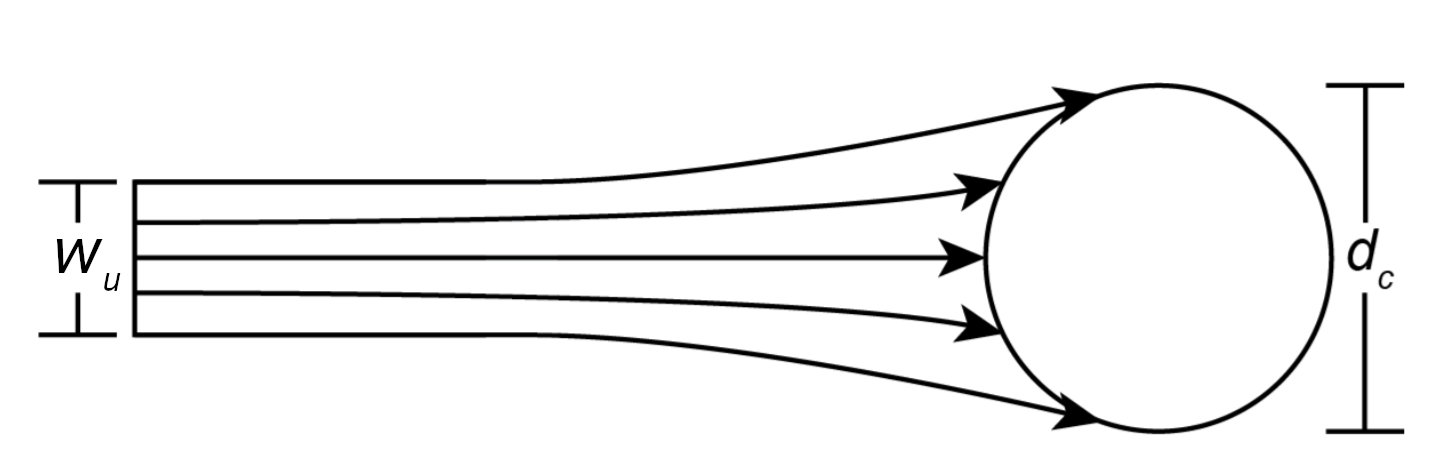
\includegraphics[width=10cm]{collectorefficiency.png}
\centering
\caption{A diagram illustrating capture efficiency for a cylindrical collector. $b$ is the horizontal width of upstream flow and $d_c$ is collector diameter. Adapted from \cite{Palmer_2004}.}
\label{fig:capeff}
\end{figure}

Particle capture in transitionally turbulent flows ($1<\Rey<1000$), which occur commonly in the environments and on the length scales of aquatic macrovegetation, does not follow the analytical expressions involving Reynolds number, collector diameter, and particle diameter ($d_p$), derived for creeping flow (REF paper that describes creeping flow solution). For transitional flows (as considered here) and turbulent flows, analytical solutions are intractable so empirical estimates are often employed. \cite{Palmer_2004} introduced a power law expression for estimating capture efficiency of cylindrical collectors, which takes the form 
\begin{equation}
    \eta=C{\Rey_c}^{a}R^{b}\,,
    \label{eq:powerlaw}
\end{equation}
where collector Reynolds number $\Rey_c=\frac{ud_c}{\nu}$, $u$ is flow velocity, $\nu$ is kinematic velocity, and $R=\frac{d_c}{d_p}$ is the ratio between collector diameter and particle diameter ($d_p$). $C$, $a$, and $b$ are empirically determined regression coefficients. It is worth noting that \cite{Palmer_2004} used $\eta$ in their notation for this model as opposed to $\eta^\prime$ because their experiment involved an isolated single cylinder coated with grease, for which retention was assumed to be complete ($p_r = 1$).

Turbulence is also theorized and empirically confirmed to affect the settling velocity of heavy, fine particles \citep{Nielsen_1993, Jacobs_2016, Wang_2018}. Particularly, turbulent eddies generated along bed roughness and within vegetation stands oppose gravitational settling of sediment particles. In addition, turbulent wakes behind individual vegetation stems can knock off sediment that has already been adhered to neighboring stems (REF paper that described this effect). Thus, sediment-vegetation interaction in transitional flow is two-fold: first, vegetation stems directly intercept sediment from the flow, and second, vegetation structure influences the flow field and its turbulence properties for gravitational settling.

\section{Previous Work}

Many previous studies on sediment capture through vegetated reaches have used laboratory flume experiments to examine the effects of different flow and vegetation conditions on the rate and efficiency of sediment removal from the water column \citep{Fauria_2015, Palmer_2004, Purich_2007,  Zhang_reconfiguration_2020, Zhang_turbulence_2020}. Laboratory flume experiments are valuable because interaction between vegetation and flow can produce complex mixing patterns and turbulence structures that require experiments to validate and describe hypotheses and theory \citep{Nepf_2012, Nepf_2008}. Sediment capture is defined as as one of the mechanisms by which sediment is removed from suspended load by vegetation stems, also referred to as collectors; capture efficiency is defined as the efficiency of collectors in removing sediment particles from suspension in water (need references on these definitions).  

Researchers have shown that vegetation stem dimensions, spatial density, and Reynolds number are important predictors of sediment transport and deposition behavior in flow through vegetated regions, particularly because of the dual effect of vegetation on increasing turbulence and drag \citep{Fauria_2015, nepf_drag_1999, Palmer_2004}. Thus, flow intensity has considerable significance in this context because its interaction with vegetation elements affects flow conditions, which in turn affect the ability of flow to entrain sediment. Sediment capture in creeping flow can be derived analytically (look up references), and many experiments have been done at the limits of laminar and fully turbulent flows to characterize sediment capture with vegetation \citep{Shan_turbulence_2020, Wu_2011, Yang_2016}. However, experiments at transitional flows are more sparse \citep{Fauria_2015, Palmer_2004, Purich_2007}. These types of flows have real-world importance because they can be typical of shallow, low-sloping wetland environments where dense vegetation cover makes vegetation-flow interactions common. Existing predictive models of sediment capture in transitional flows generally do not agree well with each other, and do not separate effects of direct capture on vegetation versus gravitational settling \citep{Fauria_2015, Palmer_2004}. In this study, we follow the strategy of previous work by using laboratory flume experiments to quantify sediment capture in vegetated reaches but build on existing studies of transitional flows by partitioning sediment capture into contributions by vegetation and gravitational settling for multiple vegetation densities and flow velocities 

\section{Hypotheses}

%what do we expect effective capture efficiency to be for transitional flows given previous work?
%are the first-order dependencies similar as those previous power law formulas?

\chapter{Methods}

%TODO
%Change method to kbackground method
%Dino's comments on methods (2020/09/15)

We conducted a suite of (x number of experiments) sedimentation experiments in a laboratory recirculating flume and used a theoretical sediment capture model to test our hypotheses. 

\section{Suspended Particle Concentration Model}

We used a sediment capture model based on that of \cite{Fauria_2015} to estimate effective capture efficiency of suspended sediment. The model follows an exponential decay of suspended sediment concentration,

\begin{equation}
    \frac{\mathrm{d}\bar{\phi}}{\mathrm{d}t} = -\left[\frac{Cv_s}{h}(1-E_r) + \eta^{\prime}ud_cI_c\right]\bar{\phi}(t) = -k\bar{\phi}(t)\,.
    \label{eq:model}    
\end{equation}

\noindent where $\bar{\phi}$ is depth-averaged suspended sediment concentration, $v_s$ is sediment settling velocity, $E_r$ is a dimensionless entrainment rate of sediment from the bed, $h$ is flow depth, and $I_c$ is the number of collectors per unit area ($I_c=\frac{N_c h}{V}$, $N_c$ is the number of collections and $V$ is the fluid volume around the collectors). The left and right summands in brackets represent the decay rate of depth-averaged suspended sediment concentration ($\bar{\phi} = \frac{1}{h} \int_0^h\phi(z)dz$) due to settling ($k_s$) and collection ($k_c$) respectively, where $z$ represents distance from the bed. $k = k_s + k_c$ is the total decay rate of suspended sediment. \cite{Fauria_2015} derived equation \eqref{eq:model} by considering vertical advection-diffusion of sediment in a flow, and assumed a Rouse profile of suspended sediment to characterize the shape of the vertical suspended sediment profile using a constant $C$. Please refer to \cite{Fauria_2015} for more details on model derivation.

The volumetric rate at which water passes through a lateral cross-section with area equal to the frontal area of one collector is calculated as $ud_ch$. The particulate mass passing through this area is found by multiplying this volume by the average mass-volume concentration ($m_p = ud_ch\bar{\phi}$). The rate at which particles are removed from suspension by this single collector is $\frac{dm_p}{dt}=\eta^{\prime}ud_ch\bar{\phi}$. By scaling up to the suite of collectors, modeled identically to one another, the change in concentration due to collection can be derived:
\begin{equation}
\frac{d\bar{\phi}}{dt} = \frac{N_c}{V}\frac{dN_p}{dt} = \frac{N_c}{V}\eta^{\prime}ud_ch\bar{\phi} = \eta^{\prime}ud_cI_c\bar{\phi}\,.
\label{eq:collection}
\end{equation}

Concentration at any height ($\phi_a$) can be assumed to be proportional to average concentration ($\phi_a=\frac{\bar{\phi}}{C}$) because we assumed the vertical profile of suspended sediment concentration maintains a steady-state shape governed by the Rouse equation in which gravitational settling of sediment is balanced by upward sediment flux due to turbulent eddies in the flow (REF Rouse). Thus, $\bar{\phi}$ in the exponential decay solution of \eqref{eq:model} can be freely interchanged with an equation of identical form for concentration at a specific height $\phi_a$,
\begin{equation}
    \phi_a(t) = \phi_a(0)e^{-kt}\,.
    \label{eq:specconc}
\end{equation}

Equation \eqref{eq:specconc} demonstrates that the sediment decay rate constants $k_s$ and $k_c$ can be modeled by measuring the time series of suspended sediment concentration at reference heights from the bed. We used this approach in our set of laboratory flume experiments to constrain the dependencies of $k_c$ and effective capture efficiency $\eta^\prime$ in a transitional turbulence regime.

\section{Experimental Methods}

\subsection{Materials}

In our experiments, we modeled the effect of flow through a stand of roughly uniformly-spaced rigid, emergent collectors on direct interception of suspended sediment. We conducted our experiments in the Ecogeomorphology flume, a laboratory recirculating flume, located in McCone Hall at the University of California, Berkeley (Figure \ref{fig:floorplan}). The flume has a 5.25 m long by 0.6 m wide open-channel section with a rectangular channel cross-sectional geometry and a smooth bed and walls. At the downstream outlet, a pump propelled water and suspended load through a pipe routing the mixture back to the upstream end of the open channel through a honeycomb flow collimator. Rotating discs in the pump entrain fluid and suspended particles through the pipe by viscous drag, minimizing any uncontrolled alteration of suspended particles outside of the open channel (REF Discflo manual explaining the principle of operation). The flume design maintains constant discharge through the open channel.

We used tap water to fill the flume to 0.4 m depth in the open channel and, for model runs with sediment, crushed walnut shell to model suspended sediment. We instrumented the flume with a number of devices:

\begin{enumerate}
    \item hoses at 3 heights above the bed (5, 14, and 27 cm) attached to peristaltic pumps to sample flume water at upstream and downstream locations,
    \item 
\end{enumerate}

(could simplify this; I think the most important part to describe the geometry like width, height, length and flow conditions in the open channel, and the fact that sediment is recirculated from downstream to upstream, also that we used tap water). In the upper part of our pump's span (span: 0-100 Hz), cavitation (i.e., taking on bubbles of air) occurred, which was accompanied by a distinct noise. This leads to greater variance in the pump's volumetric output, which translates to uncontrolled irregularity in flow velocity in the test section. To eliminate this as a confounding factor, we found the point at which it began by gradually increasing the pump's velocity while monitoring for sound. We determined that the pump ran quietly and presumably free of cavitation up to a rotation frequency greater than 30 Hz, so this value which was chosen as the maximum for our experimental treatments. (I don't think this discussion of cavitation is necessary here because we don't need to justify not using a higher flow velocity; we could move it to the supplement).

\begin{figure}[htbp]
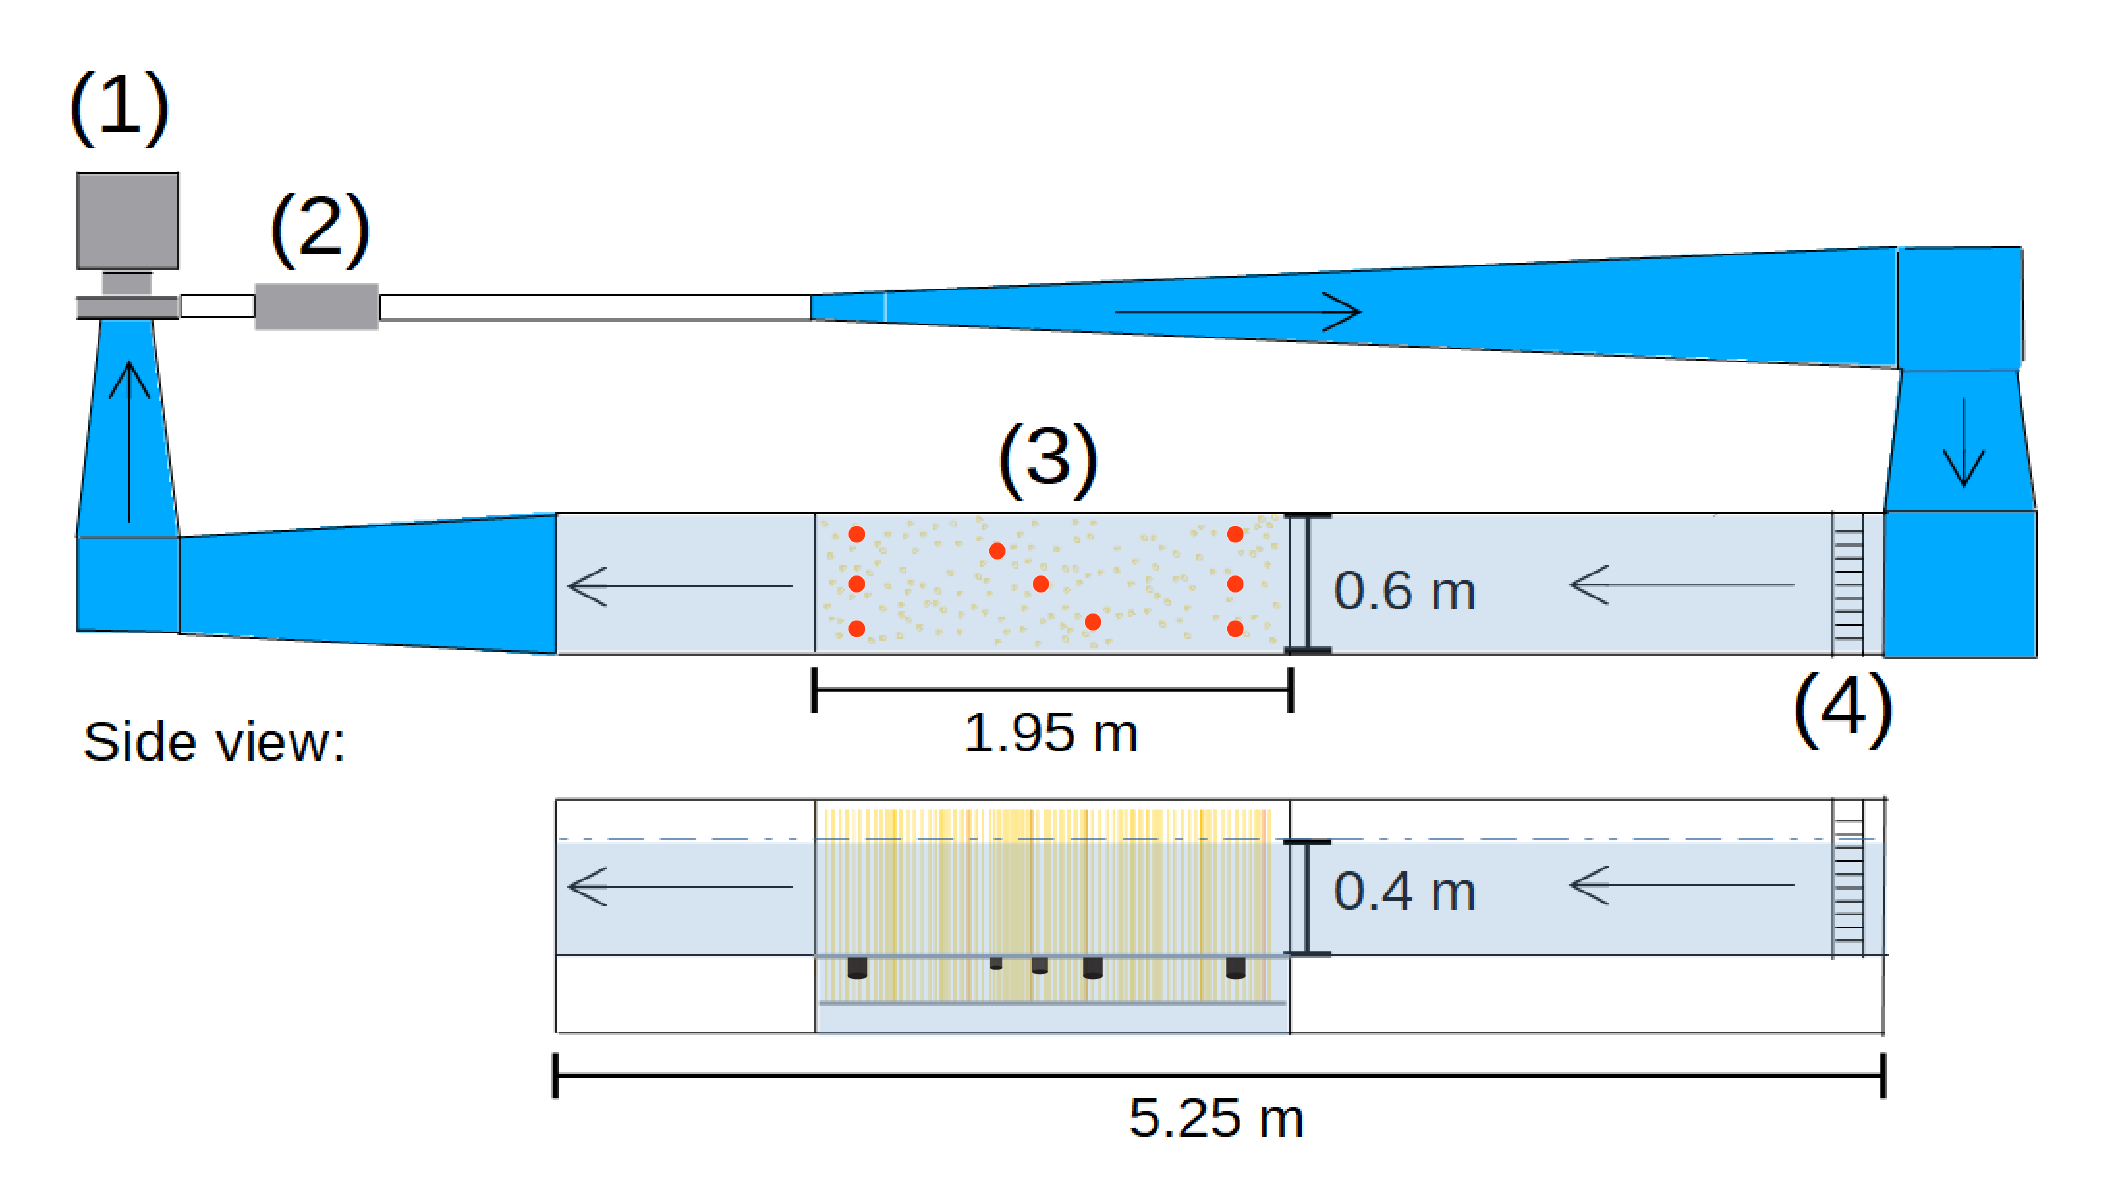
\includegraphics[width=15cm]{../pics/flume_with_sedtraps.png}
\centering
\caption{Conceptual diagram of the Ecogeomorphology laboratory flume. Labeled parts are: 1) pump, 2) magnetic flowmeter, 3) test section, and 4) honeycomb flow collimator. Arrows indicate direction of flow. A side view of the open-channel part of the system is included. Some dimensions not to scale. Red circles in the top-down view and black rectangles in the side view of the test section show the locations of the sediment traps.}
\label{fig:floorplan}
\end{figure}

We used 1/8" wooden dowels ($d_c = \SI{.3175}{\centi\metre}$) as collector stems, which were installed in a removable array that filled a recessed well in the bottom of the rectangular channel. The perforated top of the array was covered with aluminum foil, and the gap between the array and the upstream edge of the well was covered with an attached, flat, rectangular piece of aluminum in order to streamline the channel. 

Holes measuring approximately 2.5 cm in diameter were drilled in the array to hold the sediment traps. Each trap consisted of a hollow plastic cylinder with a small perforated disk affixed to the inside, on which was placed a glass microfiber filter paper to capture sediment. Nine traps were used, which were distributed throughout the test section with the goal of capturing longitudinal and lateral differences in settling should they occur (Figure \ref{fig:floorplan}).

We chose to use granular walnut shell flour to simulate sediment for our experiments because of the availability of homogeneous, sieve-measured grain sizes in suitable quantities. We performed preliminary experiments with a range of grain sizes but settled on WF5-200 as an appropriate match for sediment sizes in natural floodplains. We measured the distribution of particle size using a LISST-Portable XR laser-scattering device (Sequoia Scientific Inc, Bellevue, WA). Median particle size was determined to be approximately \SI{25}{\micro\metre} (Figure \ref{fig:sedsize}).

\begin{figure}[htbp]
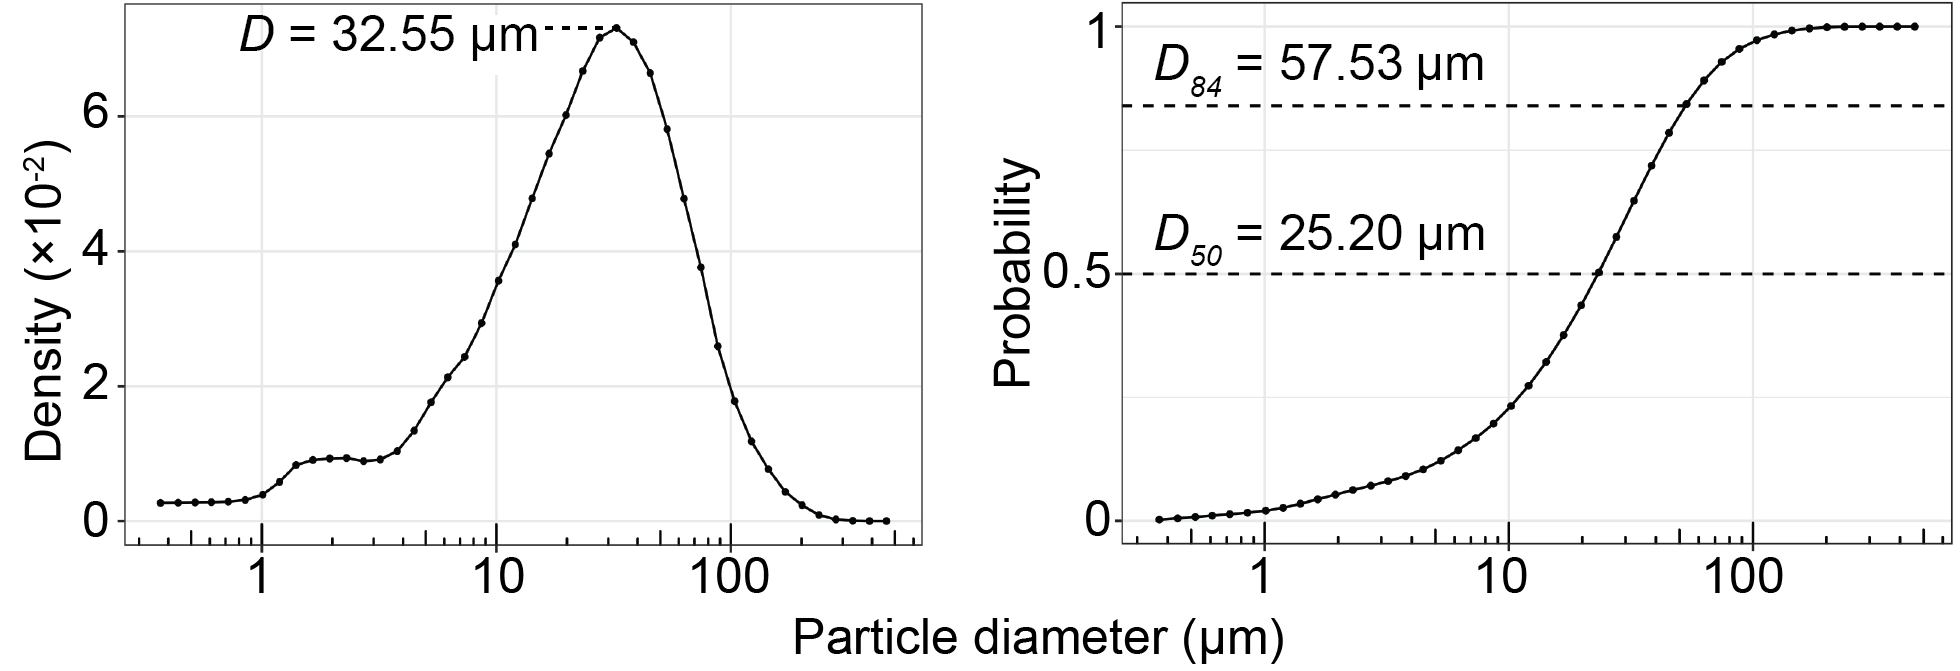
\includegraphics[width=15cm] {wf5-200sizedist.png}
\centering
\caption{Particle size distribution of WF5-200 walnut shell flour used as sediment in experiments, expressed as a probability density function (left) and cumulative density function (right). The mode of the distribution (left) and the 50th and 84th percentiles (right) are labeled.} 
\label{fig:sedsize}
\end{figure}

\subsection{Suspended Sediment Concentration Analysis}

In order to quantify the suspended particle concentration, we sampled water from the recirculating flume at regular intervals of 300 seconds throughout the duration of each experiment. Two peristaltic pumps were placed upstream and downstream of our test section, and these pumps were attached through hoses to three laterally-centered, upstream-facing inlets at heights of 5, 14, and 27 centimeters above the flume bed. The water samples from the flume were collected in plastic sampling bottles, each with around 140 mL volume capacity. The plastic bottles were cleaned between each experiment. 

We then processed the samples using vacuum filtration. Before filtration, glass microfiber filter papers were oven-dried for 24 hours at 40 degrees Celsius to remove any moisture, weighed, and assigned to a flume sample. Each water sample was run through its matching filter paper using a vacuum pump, dried once more for 24 hours, and then weighed. The resulting mass of the sediment on each filter paper was divided by the volume of its respective water sample in order to calculate the mass concentration.

The model described in section 2.2 includes only the effects of interest, which take place solely in the test section. Control runs with no collectors ($k_c = 0$) are necessary to account for the "background" decay in suspended sediment concentration due to settling in the rest of the flume ($k_{bg}$). Settling still occurs in the test section during these runs, so it was measured as usual and appears in the calculation $k_{bg} = k - k_s$. Because this rate may depend on Reynolds number \citep{Nielsen_1993, Jacobs_2016, Wang_2018}, control runs were done for each treatment level. Collector density in the test section was assumed not to affect settling outside the test section, so no duplication was performed for this parameter.

%Additionally, runs were required to estimate the entrainment rate. These were performed by adding sediment with the flume running as usual to distribute it uniformly, then turning the flume off and letting all sediment settle. At this point, a sample blank was taken. Then, the flume was turned back on and set to 30 Hz, corresponding to the highest Reynolds number of our experimental runs. 
%Not sure whether we'll dig into the constituent parts of k_s but if so, we might want to consider using the LISST since it presumably has a far lower detection limit

\subsection{Turbulence Characterization Protocols}
Continuous velocity measurements were taken with an acoustic Doppler velocimeter (ADV) at all points within our parameter space. At each point, velocity measurements were taken at 6.7, 14.8, 24.9 and 36.1 cm above the flume bed, with each measurement lasting for at least 300 seconds. The ADV measured velocity, along with other data such as autocorrelation and signal-to-noise ratio, at a frequency of 10 Hz in the $x$, $y$, and two independent measures of data in the $z$ direction. Significant differences between these two measurements help inform data quality during post processing. The instrument was positioned within the flume so that with respect to flow, $x$ denoted the longitudinal direction, $y$ the transverse direction, and $z$ the vertical direction. Before each measurement, a mixture of walnut shell flour and tap water was released into the running flume, as the particulates were needed to act as a tracer in order for the ADV to accurately detect flow velocity.
%TODO

\section{Statistical Analysis}

% should add something here about how we calculated k_total
\subsection{Settling, Capture, and Capture Efficiency}
The mass of sediment settled due to gravity was estimated by weighing oven-dried sediment trap microfiber filter papers before and after each experiment and scaling the mass of sediment by the area of the sediment trap. As there were no significant differences between sediment mass collected laterally and longitudinally with respect to flow throughout the test section, the mass settled per sediment trap area was then averaged across all nine traps. Total settling inside of the test section was calculated by scaling the average mass settled per trap area during each experiment by the area of the test section ($1.17\, m^{2}$). The rate of settling, $k_{s}$, for each experiment was then calculated with the equation \[\frac{m_{s}k}{m_{0}(1-e^{-kT})}.\] 

$k_{s}$ from each control run was subtracted from the total decay rate $k$ from the same control run to determine rate of background settling ($k_{bg}$) at each velocity in our parameter space. We calculated rate of capture, $k_{c}$, for experiments with dowels in the same manner as we calculated $k_{bg}$; however, based on the velocity of the experiment, we subtracted a corresponding $k_{bg}$ value from $k_{c}$ to account for the background settling in the rest of the flume. This new $k_{c}$ was scaled by the ratio of the volume of the entire flume to the volume of the test section. We then calculated effective capture efficiency ($\eta^{\prime}$) with Eqn. 3. 

\subsection{Turbulence and Bed Shear Stress}
Measurements taken by the ADV were filtered and despiked. Points in the time series that had low autocorrelation and points where there were large discrepancies between the two velocity measurements in the $z$ direction were excluded from analysis. Furthermore, we utilized the threshold ADV despiking algorithm detailed in \cite{goring_nikora} in order to detect spikes in the data, as well as replace these spikes using cubic interpolation.

Turbulence kinetic energy (TKE) was then calculated from the cleaned data using the equation 
\[\frac{1}{2}(<u^{'2}> + <v^{'2}> + <w^{'2}>),\]
in which, with respect to flow, $u'$ denotes velocity fluctuations in the longitudinal direction, $v'$ in the transverse direction, and $w'$ in the vertical direction. This calculation was done for each of the four heights we took measurements at in the flume, and for each Reynolds number and collector density in our parameter space. Because the velocimeter recorded three measurements simultaneously at each timepoint, TKE was calculated separately for these three measurements. 

Turbulence calculated only from the bottom-most velocity measurements taken by the ADV was multiplied by a proportionality constant $C_{1}$ (0.19) and the density of water $\rho$ in order to estimate bed shear stress ($\tau_{0}$).
\[\tau_{0} = C_{1}[\frac{1}{2}\rho(<u^{'2}> + <v^{'2}> + <w^{'2}>)]\]
Reynolds stress and a modified TKE, in which only fluctuations in the vertical direction with respect to flow are taken into account, can also be used to estimate bed shear stress; these three methods of generating bed shear stress profiles are described in Biron et al. (2004), and the method that produced the smoothest profiles, in our case bed shear stress estimated using TKE, was ultimately chosen.  


\chapter{Results}

\begin{figure}[htbp]
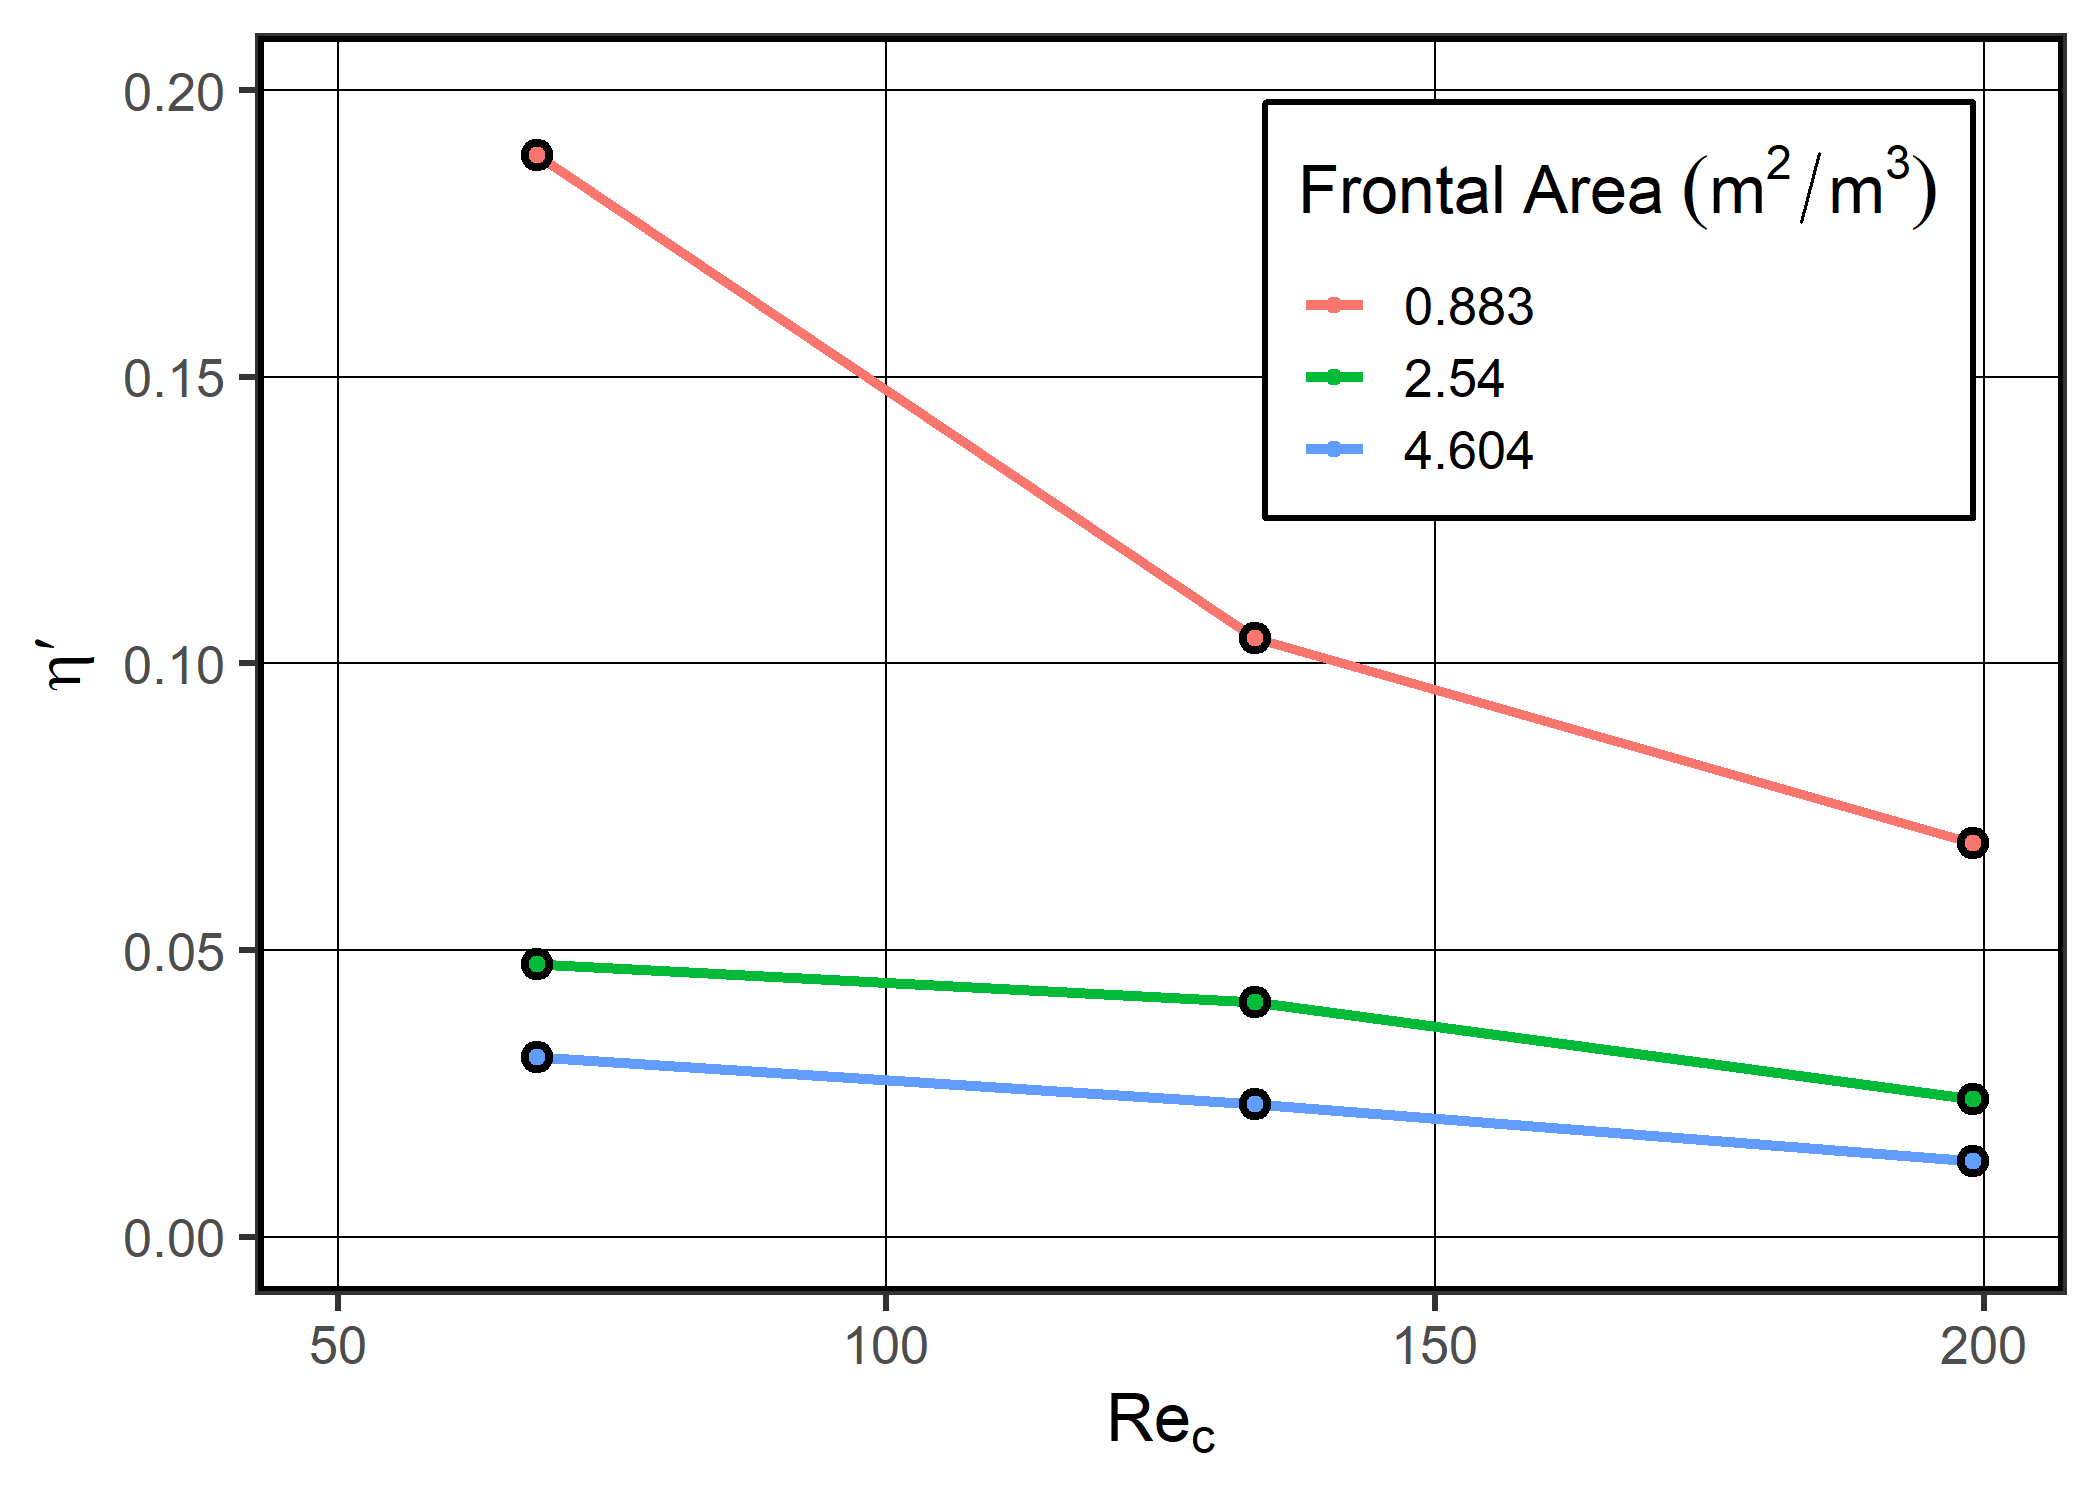
\includegraphics[width=6in]{etafig.png}
\centering
\caption{A plot showing our calculated effective collector efficiency ($\eta^\prime$) values for various values of frontal area ($I_cd_c$) and $\Rey_c$}
\label{fig:eta}
\end{figure}

\begin{figure}[htbp]
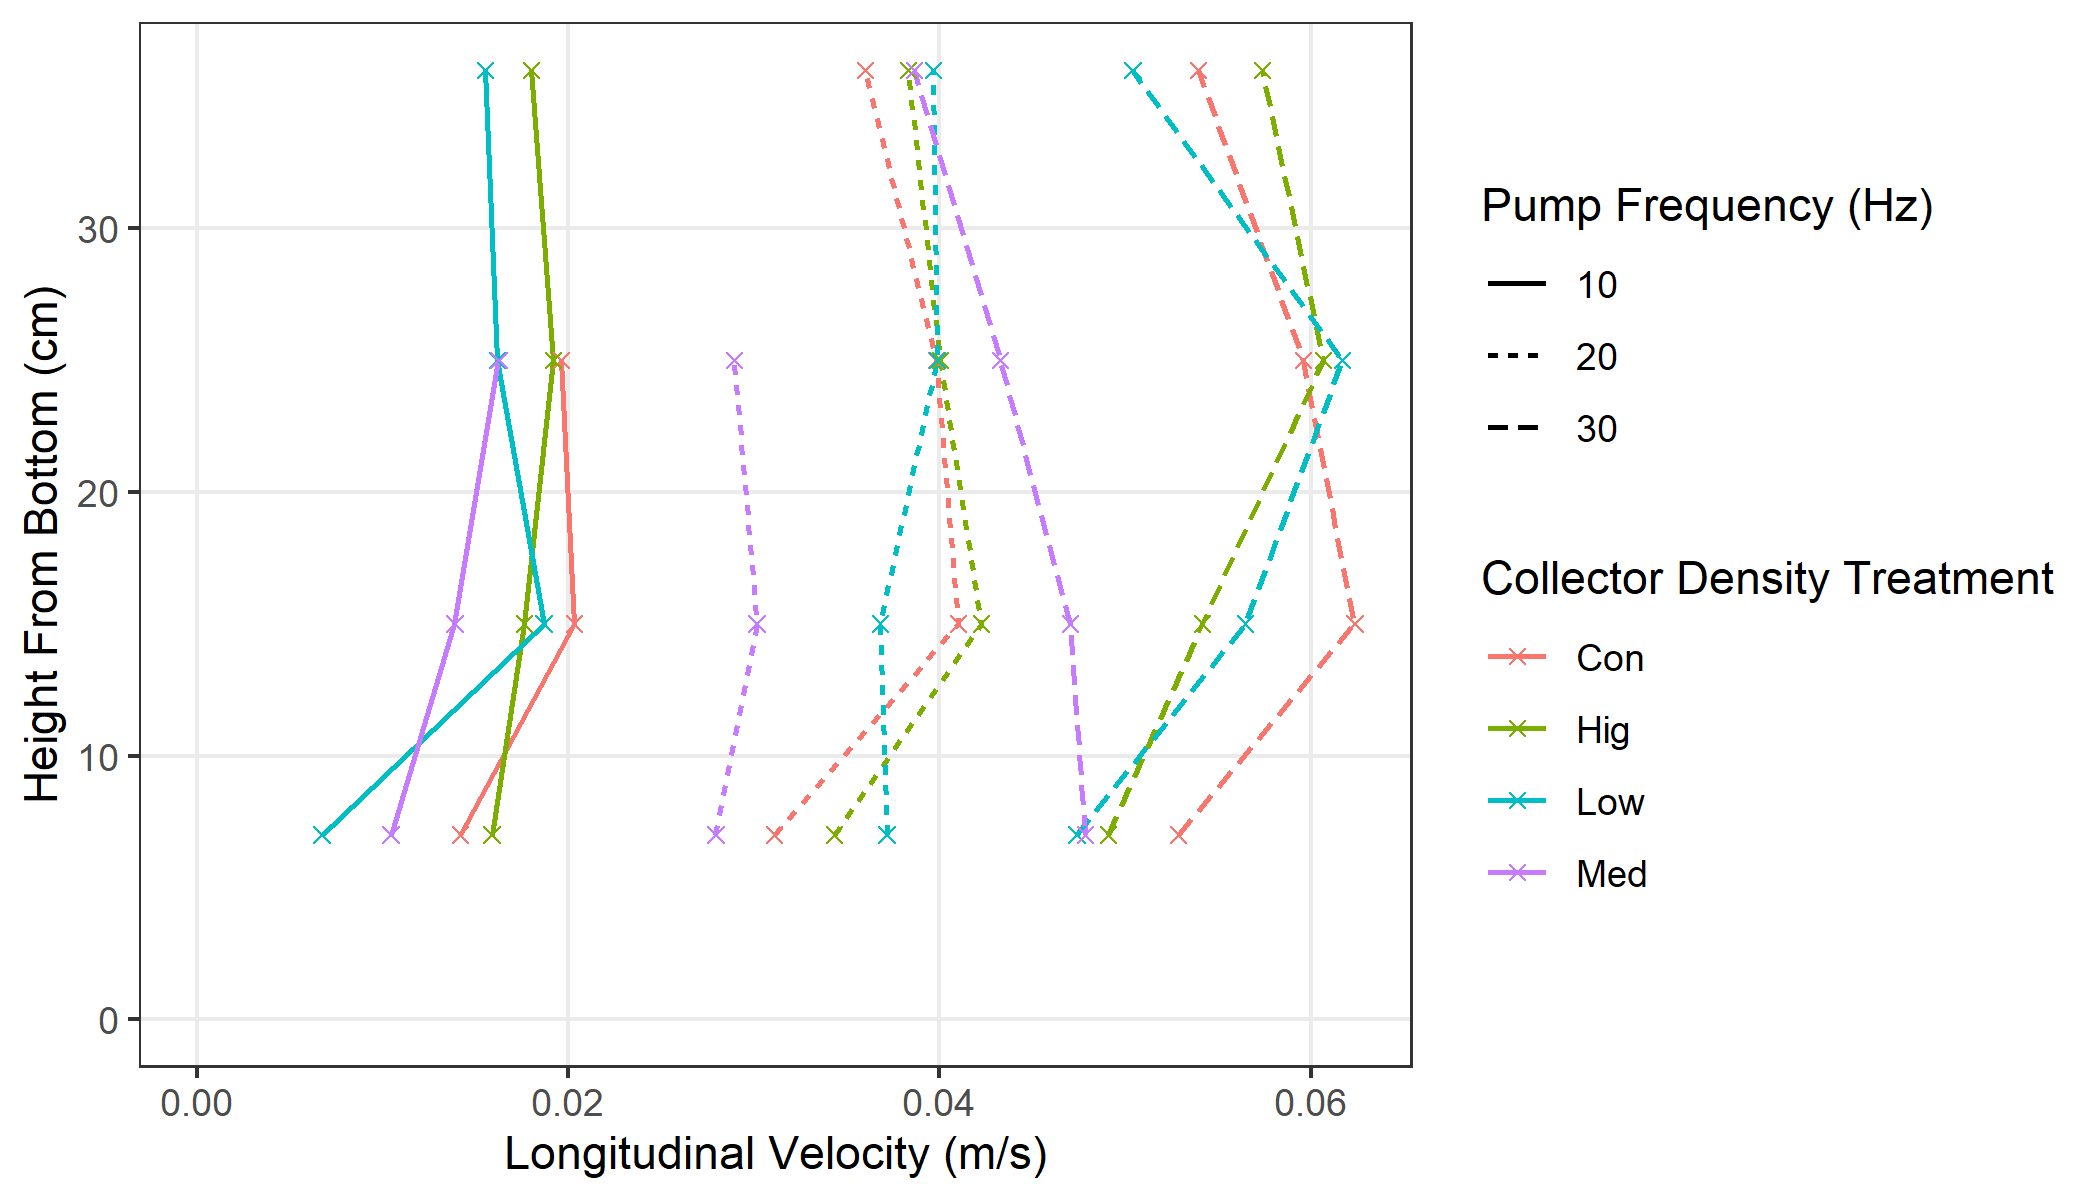
\includegraphics[width=6in]{vectrino.png}
\centering
\caption{Flow velocity profiles along the vertical axis from the bed to the water surface of the open rectangular channel for each of our collector density and Reynolds number treatments}
\label{fig:vectrino}
\end{figure}



%\chapter{Discussion}
%
%TODO
%
%The assumption that probability of retention ($p_r$) is 100\% when stems are coated with grease might be questionable based on our result that biofilm increased $\eta^\prime$ in comparison to greased dowels. The only other effect of biofilm that is readily apparent to me is perhaps increasing effective stem diameter ($d_c$). However, with our model for Reynolds number ($\Rey_c \propto d_c$), and both us and \cite{Fauria_2015} finding $\eta^\prime \sim -\Rey_c$, increasing stem diameter would be expected to have the opposite effect, unless I'm missing something.

\bibliographystyle{apalike}
\bibliography{refs}

\end{document}
